\documentclass[aspectratio=169]{beamer}

% Essential packages
\usepackage[utf8]{inputenc}
\usepackage[T1]{fontenc}
\usepackage[english]{babel}
\usepackage{graphicx}
\usepackage{tikz}

% Modern Roboto font
\usepackage[sfdefault]{roboto}
\usepackage[T1]{fontenc}

% Color definitions
\definecolor{vermelhoPrincipal}{HTML}{b11116}
\definecolor{azulComplementar}{HTML}{3a5461}
\definecolor{brancoFundo}{HTML}{FFFFFF}

% Theme configuration
\usetheme{Madrid}
\usecolortheme{default}

% Custom colors - text in black
\setbeamercolor{structure}{fg=black}
\setbeamercolor{palette primary}{bg=vermelhoPrincipal,fg=white}
\setbeamercolor{palette secondary}{bg=azulComplementar,fg=white}
\setbeamercolor{palette tertiary}{bg=vermelhoPrincipal,fg=white}
\setbeamercolor{palette quaternary}{bg=azulComplementar,fg=white}
\setbeamercolor{frametitle}{bg=vermelhoPrincipal,fg=white}
\setbeamercolor{background canvas}{bg=brancoFundo}
\setbeamercolor{title}{fg=black}
\setbeamercolor{subtitle}{fg=azulComplementar}
\setbeamercolor{author}{fg=black}
\setbeamercolor{date}{fg=black}
\setbeamercolor{itemize item}{fg=black}
\setbeamercolor{itemize subitem}{fg=black}
\setbeamercolor{enumerate item}{fg=black}
\setbeamercolor{block title}{bg=vermelhoPrincipal,fg=white}
\setbeamercolor{block body}{bg=vermelhoPrincipal!10,fg=black}
\setbeamercolor{normal text}{fg=black}

% Itemize font configuration
\setbeamerfont{itemize/enumerate body}{size=\scriptsize}
\setbeamerfont{itemize/enumerate subbody}{size=\scriptsize}

% Minimalist bullets
\setbeamertemplate{itemize item}{\raisebox{0.2ex}{\rule{0.6ex}{0.6ex}}}
\setbeamertemplate{itemize subitem}{\raisebox{0.3ex}{\rule{0.4ex}{0.4ex}}}
\setbeamertemplate{itemize subsubitem}{\raisebox{0.35ex}{\rule{0.3ex}{0.3ex}}}
\setbeamertemplate{enumerate items}[square]

% Smooth transitions
\setbeamercovered{transparent}

% Remove navigation symbols
\setbeamertemplate{navigation symbols}{}

% Custom headline
\setbeamertemplate{headline}{
  \begin{beamercolorbox}[wd=\paperwidth,ht=0.6cm,dp=0.15cm,leftskip=0.2cm,rightskip=0.4cm]{palette primary}
    \raisebox{-0.05cm}{
\includegraphics[height=0.45cm]{imgs/base/fatec-rgt.png}}
    \hfill
    \raisebox{-0.18cm}{
\includegraphics[height=0.85cm]{imgs/base/governo-sp-secretaria-logo.png}}
    \hspace{0.2cm}
    \raisebox{-0.08cm}{
\includegraphics[height=0.6cm]{imgs/base/cps-logo.png}}
  \end{beamercolorbox}
}

% Remove block shadows
\setbeamertemplate{blocks}[default]
\setbeamertemplate{itemize/enumerate body begin}{\scriptsize}
\setbeamertemplate{itemize/enumerate subbody begin}{\scriptsize}

% Custom footer
\setbeamertemplate{footline}{
  \begin{beamercolorbox}[wd=\paperwidth,ht=0.4cm,dp=0.2cm,leftskip=0.3cm,rightskip=0.3cm]{palette secondary}
    \usebeamerfont{footline}
    \insertshortauthor \hfill \hfill {\fontsize{5}{6}\selectfont\insertshorttitle} \hfill \hfill \insertframenumber/\inserttotalframenumber
  \end{beamercolorbox}
}

% Custom frame title
\setbeamertemplate{frametitle}{
  \vspace{0.3cm}
  \textcolor{black}{\insertframetitle}
  \vspace{0.1cm}
}

% Presentation metadata
\title{Classification of Manganese Deficiency in Tangerine Leaves, \\ Using Neural Networks}
\subtitle{}
\author[DSM]{ALVES, A.; FAGUNDES, L.; FREITAS, V.; RODRIGUES, J.}
\institute{Desenvolvimento de Software Multiplataforma\\FATEC Registro}
\date{\today}

\begin{document}

% Title slide
\begin{frame}
  \vspace{0.8cm}
  \begin{center}
    
\begin{tikzpicture}
      % Decorative top line
      \draw[vermelhoPrincipal, line width=2pt] (-4,0) -- (4,0);
    \end{tikzpicture}
    
    \vspace{0.4cm}
    
    {\normalsize\bfseries\inserttitle}\par
    
    \vspace{0.45cm}
    
    {\tiny\insertauthor}\par
    
    \vspace{0.1cm}
    
    {\small\textcolor{azulComplementar}{\insertsubtitle}}\par
    
    \vspace{0.5cm}
    
    
\begin{tikzpicture}
      % Decorative bottom line
      \draw[azulComplementar, line width=1.5pt] (-2.5,0) -- (2.5,0);
    \end{tikzpicture}
    
    \vspace{0.3cm}
    
    {\scriptsize\insertinstitute}\par
    
    \vspace{0.01cm}
    
    {\tiny\textcolor{azulComplementar}{\insertdate}}\par
  \end{center}
\end{frame}

% Agenda slide
\begin{frame}[b]{Agenda}
  \begin{itemize}
    \item Pitch
    \item Problem Statement
    \item Objectives
    \item State of the Art
    \item Tech Stack
    \item Materials and Methods
    \item Practical Demonstration
    \item Results and Discussion
  \end{itemize}
  
  \vfill
  
  \hfill{\scriptsize \textbf{Duration:} 10 to 11 min.}
\end{frame}

\section{Pitch}
{
\usebackgroundtemplate{%
  
\includegraphics[width=\paperwidth,height=\paperheight]{imgs/Pitch.png}%
}
\begin{frame}[b]{Pitch}
  \begin{itemize}
    \item \parbox{0.60\textwidth}{\textbf{NitrusLeaf}: Taking care of your grove!}
  \end{itemize}
  
  \vfill
  
\end{frame}
}

\section{Problem Statement}
{
\usebackgroundtemplate{%
  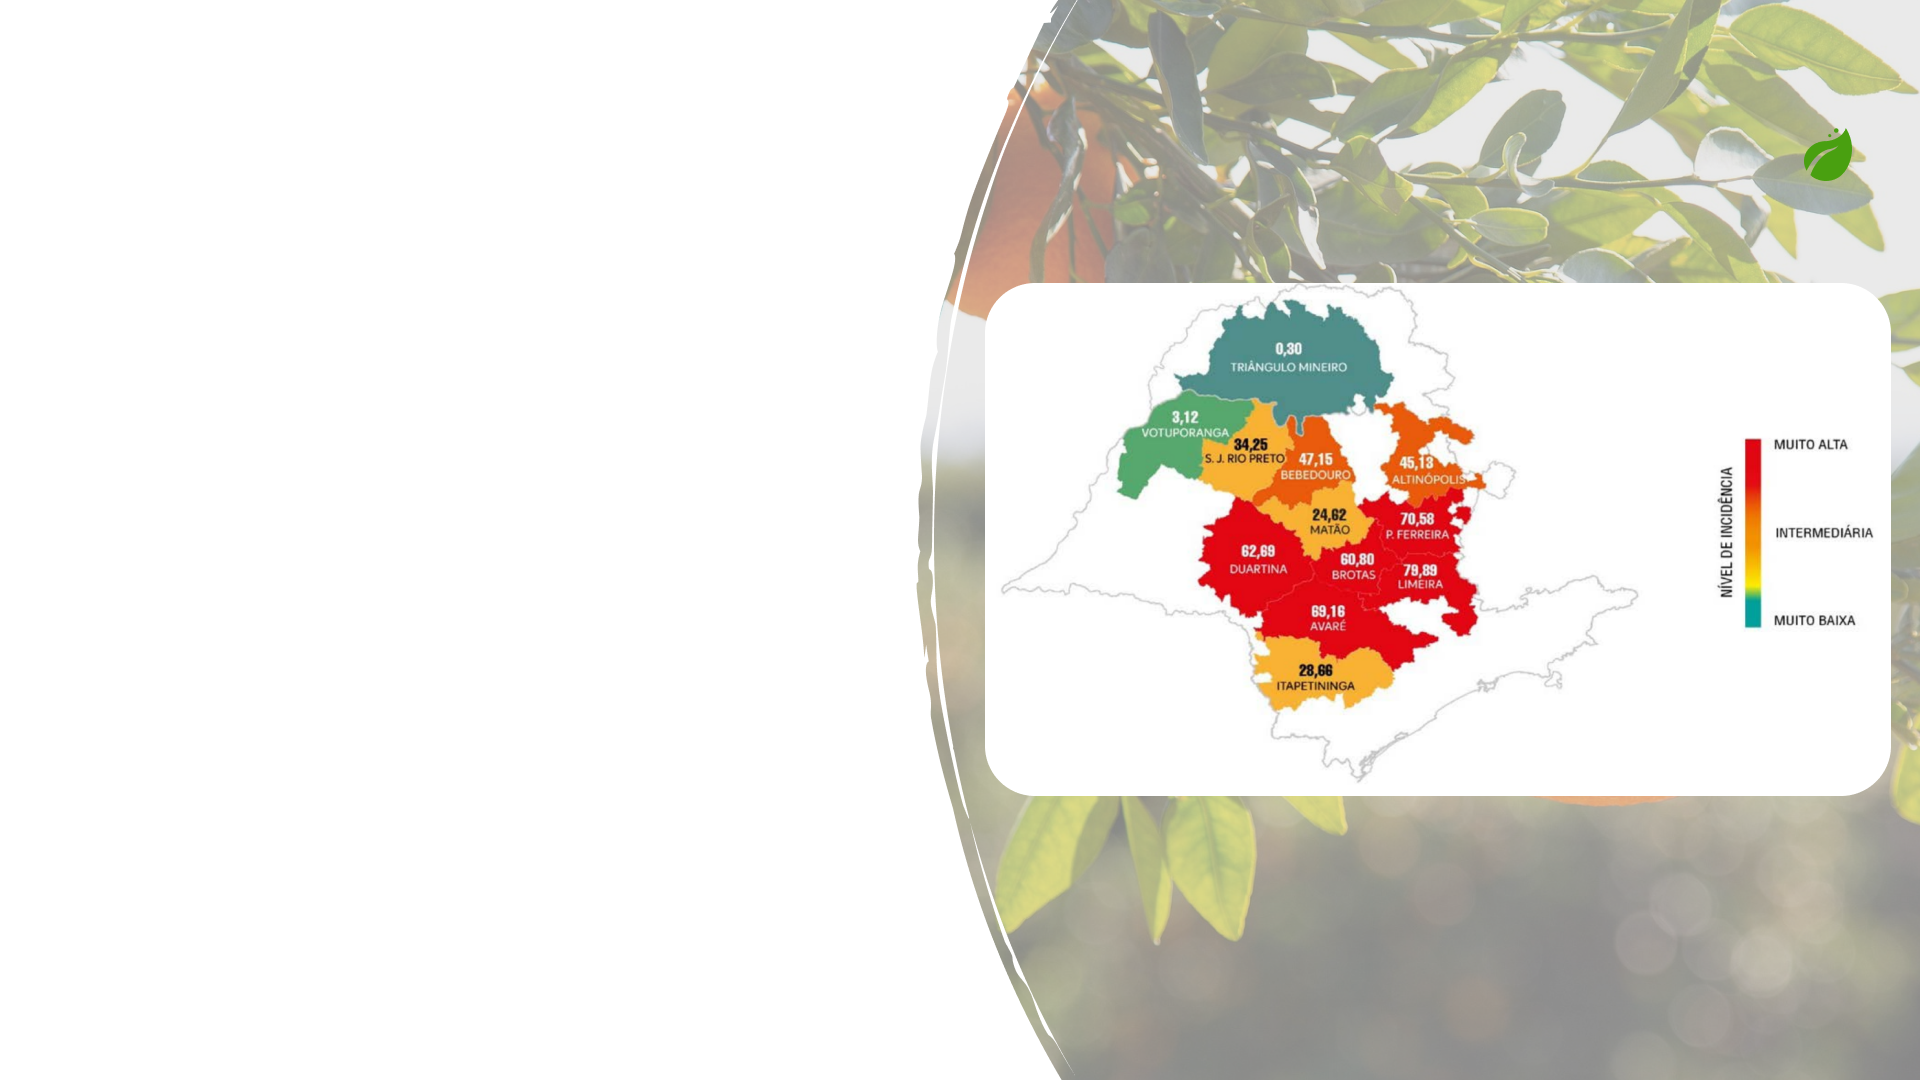
\includegraphics[width=\paperwidth,height=\paperheight]{imgs/Problematizacao.png}%
}
  \begin{frame}[b]{Problem Statement}
\begin{minipage}{0.5\textwidth}
    \begin{itemize}
        \item High incidence of citrus greening (>60\%) reported in São Paulo citrus farming.
        \vspace{0.3cm}

        \item Greening symptoms closely resemble nutritional deficiencies, complicating accurate diagnosis.
        \vspace{0.3cm}

        \item This misidentification can lead to significant crop management losses.
        \vspace{0.3cm}

        \item Smallholder farmers have limited access to reliable diagnostic tools.
    \end{itemize}
\end{minipage}
    
  \vfill
  
  {\fontsize{4}{5}\selectfont\textit{Source: Fundecitrus, Araraquara, São Paulo 2025}\hfill\textcolor{white}{Image: Percentage of orange trees affected by greening by sector and region}}
\end{frame}
}

\section{Objectives}
{
\usebackgroundtemplate{%
  
\includegraphics[width=\paperwidth,height=\paperheight]{imgs/Objetivos.png}%
}

\begin{frame}[b]{Objectives}
\begin{minipage}{0.5\textwidth}
  \begin{itemize}
    \item \textbf{General Objective}: Develop \textbf{NitrusLeaf} to identify manganese nutritional deficiency in tangerine leaves using AI.
    \vspace{0.3cm}

    \item \textbf{Specific Objectives}:
    \begin{itemize}
      \item Build a labeled image dataset.
      \item Train and validate the CNN architecture.
      \item Develop a cross-platform mobile application.
    \end{itemize}
    \vspace{0.3cm}

    \item Expected Results and \textbf{Deliverables}: A functional, accessible application with a validated AI model and an organized dataset.
    \vspace{0.3cm}
  \end{itemize}
\end{minipage}
  
  \vfill
  
  {\fontsize{4}{5}\selectfont\textit{Source: Own elaboration}\hfill\textcolor{white}{Image: AI and tangerine icon}}
\end{frame}
}

% STATE OF THE ART --------------------------------------------------------------------------------
\section{State of the Art}

% STATE OF THE ART 1
\begin{frame}[t]{State of the Art}
  \scriptsize

  Computer Vision, Machine Learning, and Deep Learning Approaches for Nutrient Deficiency Identification in Crops
  
  \vspace{0.3cm}
  
  \begin{table}
    \centering
    \tiny
    \begin{tabular}{|p{2.5cm}|p{2cm}|p{2cm}|p{2cm}|p{2cm}|p{1.5cm}|}
      \hline
      \textbf{Title/Authors} & \textbf{Objective} & \textbf{Method} & \textbf{Results} & \textbf{Limitations} & \textbf{Gap} \\
      \hline
      Computer Vision Based Machine Learning and Deep Learning Approaches for Identification of Nutrient Deficiency in Crops: A Survey - Sudhakar and Swarna Priya (2023)
      & Review computer vision techniques for detecting plant nutrient deficiencies
      & Survey of ML, DL, UAVs, IoT, and remote sensing approaches
      & CNNs, UAVs, and IoT showed strong performance in identifying deficiencies
      & High dependency on large datasets and poor generalization across varying environments
      & Lack of real-time systems and limited focus on micronutrients
      \\
      \hline
    \end{tabular}
  \end{table}
\end{frame}

% STATE OF THE ART 2
\begin{frame}[t]{State of the Art}
  \scriptsize

  Image Processing-Based Detection of Diseases and Nutrient Deficiencies in Plants

  \vspace{0.3cm}
  
  \begin{table}
    \centering
    \tiny
    \begin{tabular}{|p{2.5cm}|p{2cm}|p{2cm}|p{2cm}|p{2cm}|p{1.5cm}|}
      \hline
      \textbf{Title/Authors} & \textbf{Objective} & \textbf{Method} & \textbf{Results} & \textbf{Limitations} & \textbf{Gap} \\
      \hline
      Image Processing Based Detection of Diseases and Nutrient Deficiencies in Plants - Ghorai et al. (2021)
      & Review image processing techniques for plant disease and nutrient deficiency detection
      & Survey on computer vision, segmentation, feature extraction, and ML classifiers
      & CNNs, SVM, and hyperspectral imaging demonstrated high detection performance
      & Highly sensitive to lighting variations, image noise, and background conditions
      & Need for robust, automated, real-time systems designed for field use
      \\
      \hline
    \end{tabular}
  \end{table}
\end{frame}

% STATE OF THE ART 3
\begin{frame}[t]{State of the Art}
  \scriptsize
  
  A Comparative Study of Deep CNN in Forecasting and Classifying Macronutrient Deficiencies in Tomato Plant Development
  \vspace{0.3cm}
  
  \begin{table}
    \centering
    \tiny
    \begin{tabular}{|p{2.5cm}|p{2cm}|p{2cm}|p{2cm}|p{2cm}|p{1.5cm}|}
      \hline
      \textbf{Title/Authors} & \textbf{Objective} & \textbf{Method} & \textbf{Results} & \textbf{Limitations} & \textbf{Gap} \\
      \hline
      A Comparative Study of Deep CNN in Forecasting and Classifying the Macronutrient Deficiencies on Development of Tomato Plant - Tran et al. (2019)
      & Classify and forecast nutrient deficiencies in tomato plants using Deep Learning
      & CNNs (Inception-ResNet v2 and Autoencoder) applied to leaf/fruit images; Ensemble Averaging
      & 87.27\% accuracy with Inception-ResNet v2 and 91\% using ensemble learning
      & Limited dataset (571 images), restricted to tomatoes under controlled greenhouse conditions
      & Needs in-field validation and adaptation to other crops and micronutrient profiles
      \\
      \hline
    \end{tabular}
  \end{table}
\end{frame}

\section{Tech Stack}
{
\usebackgroundtemplate{%
  
\includegraphics[width=\paperwidth,height=\paperheight]{imgs/Ferramental.png}%
}
\begin{frame}[b]{Tech Stack}
  \begin{itemize}
      \item \parbox{0.60\textwidth}{
          \textbf{Neural Network}: Python, TensorFlow, and Keras}
          \vspace{0.3cm}
      \item \parbox{0.60\textwidth}{
          \textbf{API}: Node.js to interface the model with the client app}
          \vspace{0.3cm}
      \item \parbox{0.60\textwidth}{
          \textbf{Mobile Application}: React Native, Expo, and TypeScript}
          \vspace{0.3cm}
      \item \parbox{0.60\textwidth}{
          \textbf{Database \& Authentication}: MySQL hosted on Supabase}
          \vspace{0.3cm}
      \item \parbox{0.60\textwidth}{
          \textbf{UI/UX Prototyping}: Figma}
  \end{itemize}
  
  \vfill
  
  {\fontsize{4}{5}\selectfont\textit{Source: Own elaboration}\hfill\textcolor{white}{Image: Technology stack logos}}
\end{frame}
}

\section{Materials and Methods}
{
\usebackgroundtemplate{%
  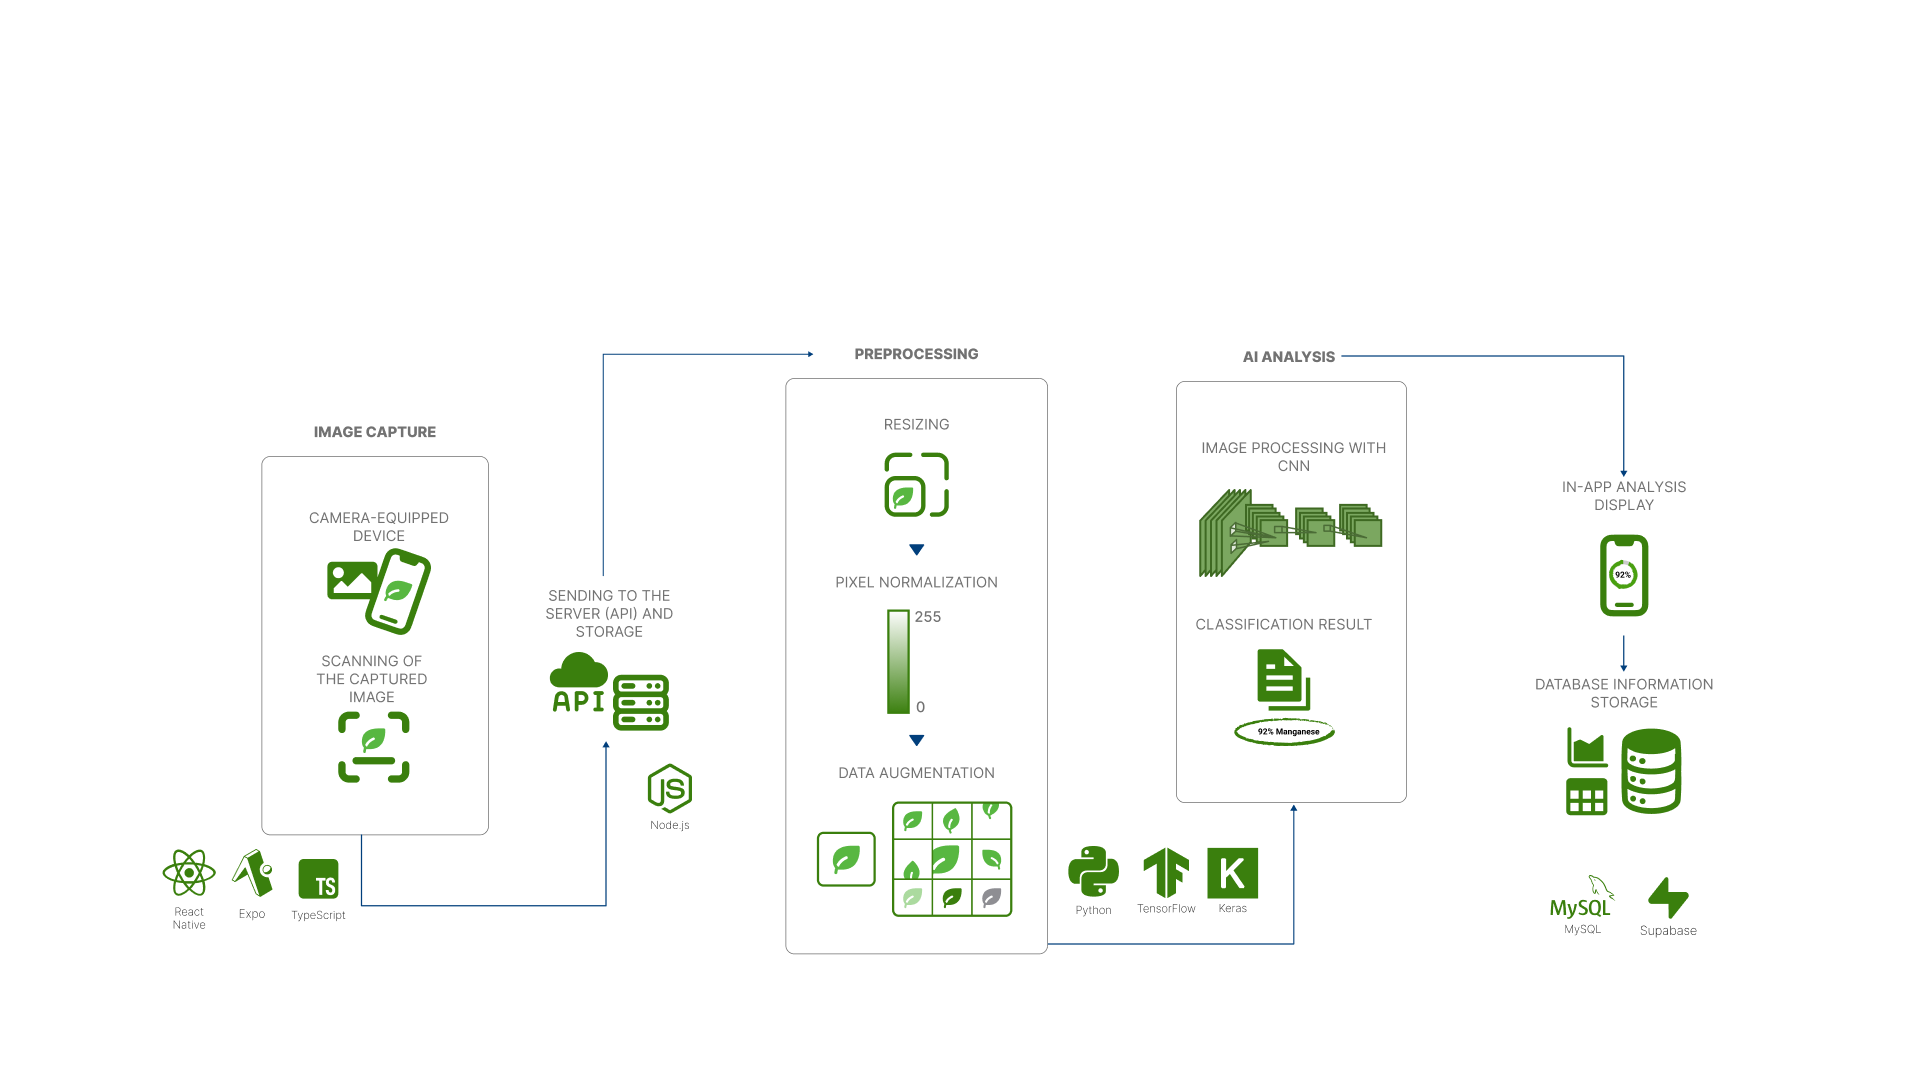
\includegraphics[width=\paperwidth,height=\paperheight]{imgs/Metodologias.png}%
}
\begin{frame}[t]{Materials and Methods}
  
  \scriptsize
  Flowchart illustrating the core processes implemented throughout the project, detailing the pipeline across Artificial Intelligence (AI) modeling and Database management.

\end{frame}
}

\section{Practical Demonstration}
{
\usebackgroundtemplate{%
  
\includegraphics[width=\paperwidth,height=\paperheight]{imgs/ApresentacaoPratica.png}%
}
\begin{frame}[b]{Practical Demonstration}
  \begin{itemize}
    \item Leaf image capture via mobile application
    \item Image dispatch to backend processing API
    \item Inference using the Convolutional Neural Network (CNN)
    \item Real-time diagnostic return
    \item Visual feedback and diagnosis display in the app
  \end{itemize}
  
  \vfill
  
\end{frame}
}

\section{Results and Discussion}
{
\usebackgroundtemplate{%
  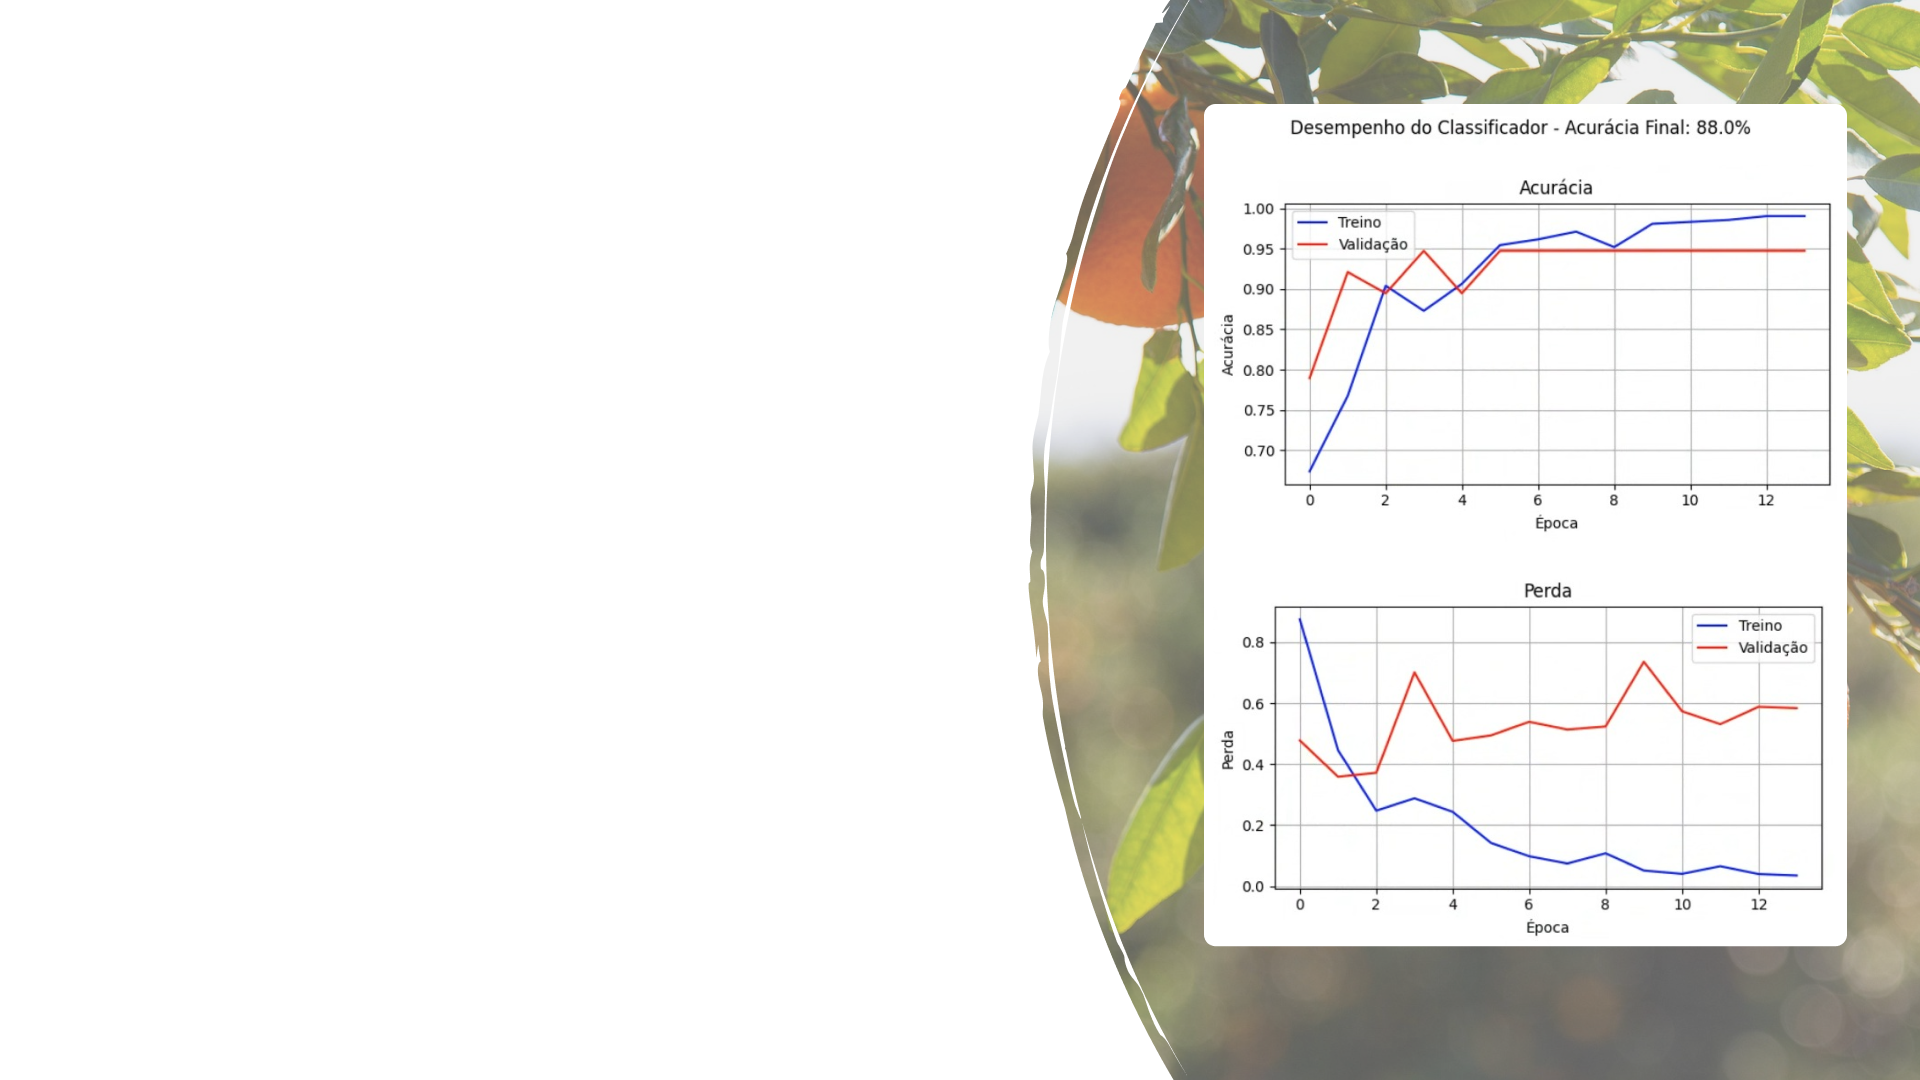
\includegraphics[width=\paperwidth,height=\paperheight]{imgs/ResultadosDiscussoes.png}%
}
\begin{frame}[b]{Results and Discussion}
  \begin{itemize}
    \item \parbox{0.5\textwidth}{\raggedright\textbf{Results}: 96\% accuracy; 24 out of 25 test images correctly classified (healthy vs. manganese-deficient leaves).}
    \vspace{0.45cm}
    \item \parbox{0.4\textwidth}{\raggedright\textbf{Limitations}: Constrained sample size and high sensitivity to ambient illumination and camera capture conditions.}
    \vspace{0.45cm}
    \item \parbox{0.4\textwidth}{\raggedright\textbf{Next Steps}: Expand dataset volume, perform in-field testing, evaluate alternate CNN architectures, and incorporate copper deficiency.}
  \end{itemize}
  
  \vfill
  
  {\fontsize{4}{5}\selectfont\textit{Source: Own elaboration}\hfill\textcolor{white}{Image: Leaf classification model performance metrics}}
\end{frame}
}

% Closing slide
{
\usebackgroundtemplate{%
  
\includegraphics[width=\paperwidth,height=\paperheight]{imgs/Obrigado.png}%
}
\begin{frame}[b]{}
  % \vspace{0.2cm}
  
  % \hspace*{0.25\paperwidth}{\Large \textbf{Thank you for your attention!}}
  
  % \vfill
\end{frame}
}

\end{document}